\section{Approach}

Our approach replaces weights with priority scheduling.

Enforcing priorities requires fewer global runqueue searches than weights,
because searches only need to happen on \textit{class boundary crossings}: on
\exit{}, when switching to running a low-class process, and on \entry{}, when
enqueueing a high-class process. These checks ensure that a core running a BE
thread $t$ knows there are no queued LC threads anywhere: the \exit{} check
ensures there's none when starting to run $t$, and the \entry{} check ensures if
one wakes up while running $t$, it will interrupt $t$.

\begin{figure}[t]
    \centering
    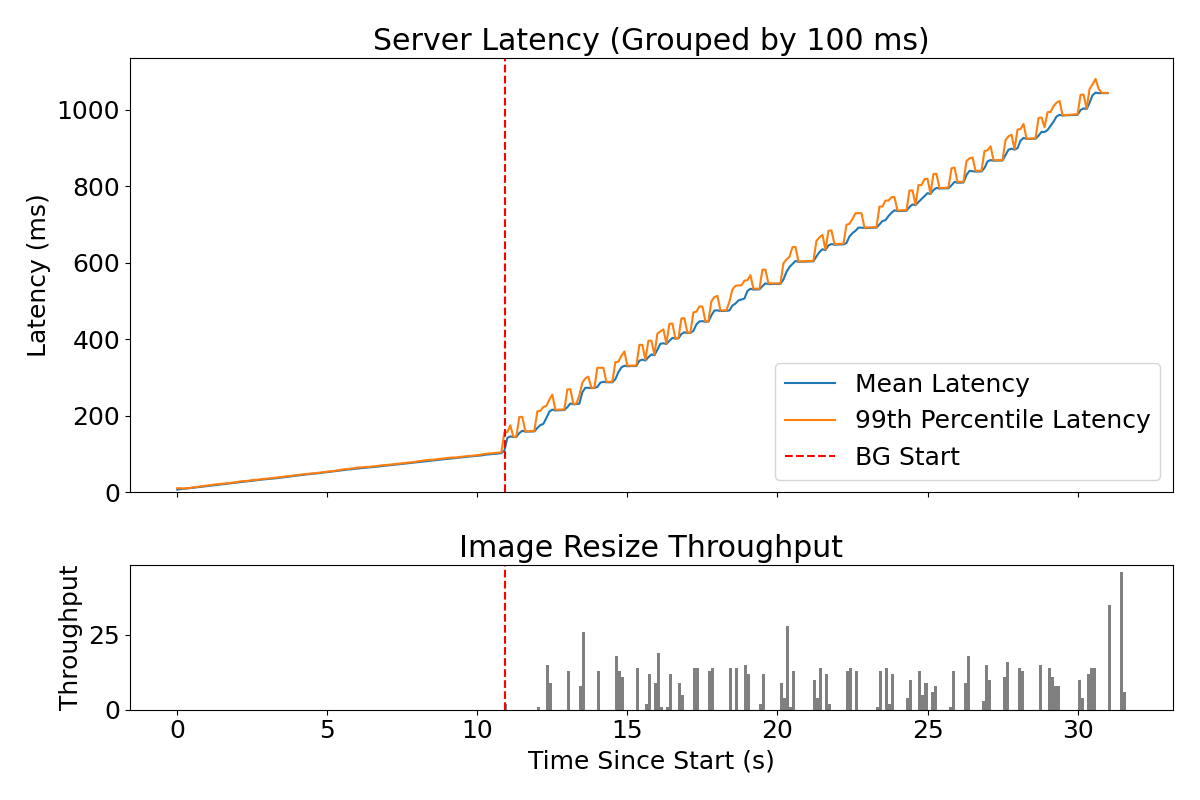
\includegraphics[width=0.9\columnwidth]{graphs/overload-rt.png}
    \caption{when running the server in real time, throttling degrades
    performance at high load}\label{fig:overload-rt}
\end{figure}
% when running the server in real-time, throttling degrades
%     performance at high load


Linux enforces priority across scheduling classes, but higher class schedulers
are designed for real-time applications. Additionally, Linux throttles them
under high load in order to not starve the default class. We see this
happening in \autoref{fig:overload-rt}, where throttling leads to spikes in the
BE's throughput and corresponding spikes in the server's latency.

We design a new scheduling class \beclass{} that sits at a lower priority than
the default one, and enforces LCs' uncontended access to reserved CPUs. To
enforce reservations under high load, without throttling LCs or killing BEs,
\beclass{} uses \textit{parking}, wherein user-space code never runs, only
kernel-level services. We implement this strict priority in Linux.